\chapter{Introducció}

Des de l'aparició dels primers videojocs, la seva evolució ha estat sempre emparellada amb una evolució tecnològica constant i, en certs punts, accelerada. Aquesta evolució tecnològica no només consta de millores en el rendiment i qualitat de cada joc sinó que, a més, s’han aconseguit generalitzar solucions i aplicar la tecnologia d’un videojoc a d'altres i fins i tot crear eines que permeten el desenvolupament de jocs a partir d'elles.

Si mirem aquesta evolució des de més a prop, veiem com al principi els videojocs eren evolucions d'altres jocs típics de bar, màquines escurabutxaques com el pinball serviren d'inspiració per a crear els primers videojocs comercials, amb un model de negoci molt semblant. Posteriorment, la necessitat de crear grans quantitats de jocs va obligar als desenvolupadors a crear màquines que poguessin executar més d'un joc i així abaratir costos i finalment, amb l'arribada dels ordinadors personals i les consoles de sobretaula, es comença a desenvolupar un mercat per a jocs sobre plataformes genèriques.

A poc a poc van apareixent els motors gràfics - programes o mòduls encarregats del renderitzat d'un joc o d'un programa amb gràfics 2D o 3D - o fins i tot motors de joc - una plataforma per desenvolupar-hi un joc a sobre -. En un principi aquests motors s'utilitzaven dintre de la mateixa companyia que el creava. Per exemple LucarArts creà {SCUMM} ({Script Creation Utility for Manic Mansion}) \citep{WikiScumm} a l'hora que creava la seva aventura gràfica de "Point \& Click" Manic Mansion (1987). Aquest mateix programa fou utilitzat després en d'altres jocs com Indiana Jones i l'Última Creuada, LOOM, El Dia del Tentacle i tres jocs de la saga Monkey Island (fins al 1998).

Un pas més endavant el va dur Id Software amb el seu {\em id Tech}  \citep{WikiScumm}. Aquest motor - i les seves evolucions - no només es feu servir per fer jocs com Doom (1993) i Doom II (1994) d'Id Software, sinó que es va vendre a altres companyies per a fer altres jocs, tot i que aquests jocs serien molt semblants al Doom original, com serà el Half-Life(1998) basat en el Quake engine, una evolució de l'{\em id Tech}. Posteriorment fins i tot hi va haver companyies que basaven el seu negoci no en vendre jocs, sinó en vendre motors a altres companyies que els fessin servir; és doncs l'aparició definitiva dels motors com a Middleware.

Paral·lelament a l'evolució tecnològica ja esmentada, la metodologia de desenvolupament i els mateixos llenguatges de programació han anat evolucionant. L'evolució més important fou quan es va passar de programar bàsicament en {\bf C} a {\bf C++}. El canvi de paradigma, però, s'ha demostrat difícil i, tot i que l'ús de la metodologia orientada a objectes és predominant a quasi totes les àrees d'un motor, encara n'hi ha alguna on porta problemes.

El cas més important, i el que en aquest treball ens centrarem és en la definició de la lògica d'un joc.

\section{Evolució en les mecàniques dels jocs}

Les lògiques dels jocs, també conegudes com a mecàniques, són les normes que defineixen els jocs. Aquestes normes estan compostes per diversos elements, que interactuen entre ells de forma més o menys complexa. En aquesta secció explicarem l'evolució que han anat prenent els mètodes que tenen els desenvolupadors per a definir aquestes normes; des d'una aproximació jeràrquica i intuïtiva, agrupant els elements per característiques comunes, fins a una de menys intuïtiva, però més flexible, on cada comportament es defineix de forma independent i cada element agafa aquells comportaments que li interessen.

\subsection{L'aproximació clàssica}

Quan un programador de {C++} o de qualsevol llenguatge orientat a objectes s'asseu davant el desafiament de programar la lògica d'un joc, trenca els diferents objectes que el poblen i els distribueix en diferents grups i subgrups, després en programa les funcionalitats comunes i acaba creant una jerarquia de classes que defineixen tots els objectes i les seves interrelacions. 

Aquesta aproximació sembla senzilla, però acaba comportant diversos problemes. Com s'explica a \citep[p.~719]{Gregory09}, les jerarquies massa grans d'objectes pateixen dels següents inconvenients:


\begin{figure}
  \centering
  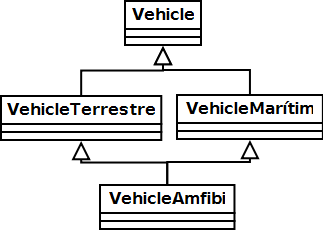
\includegraphics[width=0.58\linewidth]{./img/RombeMort.png}
  \caption{Diamant de la mort \label{fig:RombeMort}}
\end{figure}

\begin{itemize}
  \item {\bf Manteniment} \hfill \\
    A més profunda és una classe dintre d'una jerarquia, més costa d'entendre, mantenir i modificar, ja que s'ha d'entendre tant ella com totes les seves classes superiors. Així com modificar una classe mare pot comportar problemes  a classes derivades molt difícils de detectar i arreglar.
    
  \item {\bf Impossibilitat de descriure taxonomies multi-dimensionals} \hfill \\
    Crear classes en forma d'arbre és molt pràctic i sobretot intuïtiu, especialment on a cada nivell es fan separacions respecte un criteri per cada nivell. El problema seriós arriba quan ens trobem amb classificacions que no havíem previst inicialment. Per exemple podríem haver classificat 2 tipus de vehicles: vehicles terrestres i marítims, per posteriorment haver d'afegir vehicles amfibis, repte que ens porta als 2 següents punts.
    \begin{enumerate}
      \item {\bf Herència múltiple. El diamant de la mort} \hfill \\
        La solució naïf del problema anterior seria crear la classe {\em VehicleAmfibi} hereva tant de {\em VehicleTerrestre} com de {\em VehicleMarítim}, cosa que ens porta directament a l'herència múltiple. Com s'explica a \cite[p.~2]{Martin97}, l'herència múltiple causa diversos problemes, moltes vegades més grans que aquells que soluciona. En aquest cas veuríem que la classe {\em VehicleAmfibi} heretaria dues vegades {\em Vehicle}, amb els problemes d'ambigüitat que això duria (figura \ref{fig:RombeMort}).
        
      \item {\bf Classes Mix-in} \hfill \\
        Una altra solució per crear taxonomies multi-dimensionals és crear un seguit de classes que aportin funcionalitat a diversos llocs de la jerarquia. Aquestes classes, per funcionar bé, cal que siguin heretades només per les fulles i que cap d'elles tingui una classe mare. Per tant diríem que una classe només pot tenir un "avi" en qualsevol cas. Aquesta solució comporta, sobretot, molta disciplina i acaba resultant en una solució molt semblant a "agregar" funcionalitat en comptes d'heretar-la.
        
    \end{enumerate}
  \item {\bf Efecte bombolla} \hfill \\
    A l'inici del disseny, les classes arrels - les més pròximes a l'inici de la jerarquia - són dissenyades inicialment amb poca funcionalitat. A mesura que avança el projecte, i davant del desig de compartir codi i, sobretot, no duplicar-lo, molta funcionalitat va pujant a la jerarquia fins que troba el \"{}comú denominador\"{}. A poc a poc, les classes arrels es van fent pesades fins que contenen la major part de funcionalitat, que les seves filles s'han d'encarregar d'activar correctament. Col·lateralment això fa que moltes classes acabin tenint una funcionalitat i unes variables que realment no necessiten, fent que el programa usi més memòria de la necessària, un problema especialment greu en jocs de consola, on la memòria és un bé molt escàs.
    
\end{itemize}

Per a més informació sobre els defectes d'aquesta estructura, consultar \cite{Wilson02}.

\subsection{De l'{\em és-un} al {\em conté-un}}


La primera millora, o petit canvi, que es proposa respecte l'aproximació anterior, és agregar la funcionalitat en comptes d'heretar-la. Si volem crear un objecte amb moviment, que es renderitzi, que col·lisioni i que s'animi - un enemic, per exemple -, abans heretaríem d'una jerarquia on, més amunt o més avall, estigui implementada tota aquesta funcionalitat (figura \ref{fig:EnemicHerencia}). Ara, però, el que hauríem de fer és simplement crear un seguit de propietats a la classe {\em Enemic} que apuntin a instàncies d'altres classes que ens aportin cada una la funcionalitat que busquem (figura \ref{fig:EnemicAgregacio}).

\begin{figure}
  \centering
  \subfloat[Estructura per herència]{\label{fig:EnemicHerencia}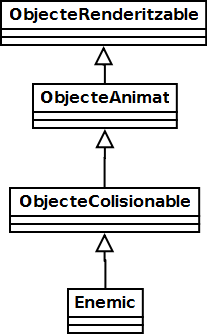
\includegraphics[width=0.23\textwidth]{./img/EnemicHerencia.png}}
  \hspace{0.08\textwidth}
  \subfloat[Estructura per composició]{\label{fig:EnemicAgregacio}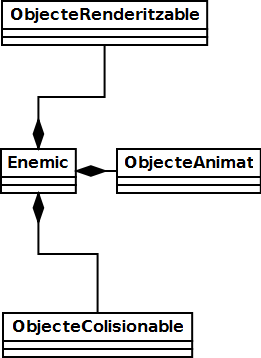
\includegraphics[width=0.27\textwidth]{./img/EnemicAgregacio.png}}
  \caption{Comparació d'herència i composició. \label{fig:HerenciaAgregacio}}
\end{figure}

Dintre d'aquest esquema, les classes que aporten funcionalitat són moltes vegades anomenades {\em Components} o {\em objectes-servidors}, ja que són les que componen els objectes finals.

Aquesta aproximació millora en certs aspectes l'anterior, però encara té alguns inconvenients. Es tendeix a tenir una classe {\em GameObject} amb un punter a cada tipus de component, al qual se li afegeixen o treuen els components segons convingui - un {\em Enemic} contindrà el component {\em ObjecteAnimat} mentre que una {\em Habitació} no -; cosa que comporta primer el problema de qui s'ha d'encarregar de destruir els components - evident fins que arribes al punt que vols substituir un component en temps d'execució - i després la pèrdua d'eficiència que comporta haver de comprovar constantment si una instància conté o no cada component per fer-ne operacions.

Un pas més enllà es troba l'aproximació on cada tipus de {\em Component} implementa una interfície comuna molt bàsica i després el {\em GameObject} simplement conté un array dinàmic que els conté tots, i crida les seves funcions ordenadament. Aquesta aproximació comporta sovint el problema de que els components cal ordenar-los, ja que moltes vegades la seva funcionalitat no és commutativa.

Un últim pas en aquesta línia és eliminar per complet el {\em GameObject} i tenir arrays de components i lligar-los simplement per l'índex; Arrays o una implementació menys costosa en memòria com Taules Hash. Aquesta aproximació sovint anomenada com a {\em Model de Components Pur} guanya sobretot en coherència de cachè. Normalment tots els components d'un tipus s'actualitzen alhora, en estar tots en un array seguits, els {\em misses} de cachè són mínims.

Finalment, un gran avantatge d'un sistema d'aquest tipus és, com s'explica a \citep{Leonard99}, la possibilitat de, un cop definits els tipus de components i les seves propietats, crear un \"{}editor del joc\"{} que permeti, amb l'ajuda d'una interfície gràfica, crear, manipular, modificar, afegir, treure, etc. objectes i components del món de forma molt senzilla. Una eina d'aquestes característiques disminueix la dependència que hi ha entre dissenyadors i programadors i permet que cada un d'ells pugui fer la seva feina en paral·lel de la forma més eficient possible.

\subsection{De centrar-nos en els objectes, a centrar-nos en les propietats}

L'últim pas, que abstreu totes les idees anteriorment exposades, és trencar totalment l'esquema orientat a objectes. La clau aquí és oblidar que un objecte està format per un seguit de propietats i mètodes, i quedar-se només amb les propietats. D'aquesta manera podem crear una taula per cada tipus de component que un objecte del joc pot tenir, i fer-ne una columna per cada propietat i una fila per cada objecte que el contingui, tenint cada objecte del joc, el que abans coneixíem com un {\em GameObject}, un identificador únic.

Aquesta aproximació no està pas mancada de defectes, i cal tenir-los en compte. El primer d'ells és la dificultat que hi ha d'establir relacions entre les {\em entitats} del joc, ja que no existeix una implementació en sí, d'aquesta entitat. Relacionat amb això hi ha el problema d'inicialitzar aquestes {\em entitats}, que s'ha de fer d'una forma més o menys aliena al mateix sistema. Finalment, el dilema més gran, és decidir on es programa el comportament de les entitats, i hi ha bàsicament 2 solucions, amb les seves variants:

\begin{enumerate}
  \item {\bf Dintre els mateixos components} \hfill \\
    Cada propietat porta incorporada la seva funcionalitat d'alguna manera. Sigui directament dintre del mateix component, via mètodes en aquest - cosa que retorna a la metodologia orientada a objectes - o via els anomenats {\em sistemes}. Aquests s'encarreguen de recollir aquelles {\em entitats} que reuneixen unes condicions - normalment, tenir un o més components - i actualitzar-los.
    
  \item {\bf Via components especials} \hfill \\
    En aquesta variant normalment es defineix un tipus especials que simplement conté un apuntador - o referència equivalent - a un script que implementi una interfície coneguda i que defineixi el comportament d'aquesta entitat.
    
\end{enumerate}

Si ara ens centrem en els problemes que tenia l'aproximació clàssica i ho comparem amb aquesta nova aproximació, ens trobem amb les següents millores:

\begin{itemize}
  \item {\bf Manteniment} \hfill \\
    En aquest cas, els problemes de manteniment no s'han esvaït del tot, sinó que s'han traslladat. Ara no hi ha cap problema per entendre jerarquies complexes, doncs aquestes s'han esvaït, i cada funcionalitat s'ha separat, així que és més fàcil de comprovar si funcionen correctament. Però la combinació d'aquestes i les seves interconnexions poden dur més d'un problema difícil de detectar.
    
  \item {\bf Impossibilitat de descriure taxonomies multi-dimensionals} \hfill \\
    Aquest problema queda completament resolt, doncs cada entitat agafa la funcionalitat que vol i no està obligada a pertànyer a cap grup. Mirant el problema descrit anteriorment de tenir definits vehicles terrestres i vehicles aquàtics, i voler-ne afegir d'amfibis, ho solucionaríem de la següent manera:
    \begin{enumerate}
      \item Definim com a vehicle terrestre tota aquella entitat que contingui el component \"{}vehicle terrestre"
      \item Definim com a vehicle aquàtic tota aquella entitat que contingui el component \"{}vehicle aquàtic\"{}.
      \item Definim com a vehicle amfibi tota aquella entitat que contingui els components \"{}vehicle aquàtic\"{} i  \"{}vehicle terrestre\"{}.
    \end{enumerate}
    
    Possiblement calgui modificar els components \"{}vehicle aquàtic\"{} i  \"{}vehicle terrestre\"{} tals que puguin operar a l'hora, però aquesta modificació no serà molt complexa.
    
  \item {\bf Efecte bombolla} \hfill \\
    Aquest problema desapareix totalment. Si detectem que 2 o més components tenen funcionalitat comuna, el més assenyat en aquest cas és crear un nou component amb aquesta funcionalitat i treure-la dels anteriors. Així només hem de vigilar que les entitats tinguin tots els components que necessiten i mai una entitat tindrà més informació o funcionalitat de la estrictament necessària.
    
\end{itemize}

\subsection{Definició}

Finalment diríem que un sistema d'entitats és aquell {\bf sistema} que regeix el comportament d'un seguit d'{\bf entitats}, definides a partir d'uns {\bf components}. Cada entitat té associat com a màxim un component de cada tipus. El comportament d'aquestes entitats ve únicament regit per quins {\bf components} té associats i les dades que aquests contenen.

\section{Implementacions}

En aquesta secció farem un repàs de diverses implementacions de sistemes d'entitats que s'han fet anteriorment, analitzarem les seves característiques i els avantatges i inconvenients d'alguns.

Començarem amb un anàlisi d'alguns jocs que han seguit aquesta aproximació, seguidament parlarem de motors de jocs i finalment parlarem del nostre motor, i quines característiques tindrà que el diferenciïn dels anteriors.

\subsection{Jocs Concrets}

És difícil de rastrejar quins jocs tenen una estructura d'agregació en comptes d'herència, ja que moltes vegades no es fa pública la implementació d'aquestos. Però gràcies als anomenats {\em postmortemps} (Documents que s'escriuen un cop finalitzat un joc, on se n'analitza el desenvolupament, es busquen quines coses han anat bé i quines no i s'intenta fer auto-crítica de cara a millorar el desenvolupament dels següents projectes) en tenim accés a alguns.

\begin{description}
  \item[Thief] \citep{Leonard99} \hfill \\
    Potser un dels exemples més antics, encara que segurament no el més antic, ja que el sistema és sempre una evolució d'algun motor usat anteriorment. Basa la seva força en facilitat d'edició mitjançant GUIs i una alta versatilitat, desenvolupant 2 jocs en paral·lel bona part del temps ({\em Thief} i {\em System Shock 2}). Es destaca que en aquests jocs no hi ha cap jerarquia d'objectes en el codi, sinó que tota es crea a partir de dades.
    
  \item[Tony Hawk's Pro Skater 3] \citep{West07} \hfill \\
    En aquest exemple veiem la necessitat d'una companyia de treure jocs amb una alta freqüència (un a l'any) i com, a poc a poc evolucionant cap a un sistema d'entitats fetes amb agregació de components. El canvi de jerarquies en el codi a objectes creats via dades fou lent i al principi contraproduent, però 2 anys després de començar el canvi els resultats es feren evidents, on el joc va guanyar en velocitat d'execució i els creadors en temps de producció.
    
  \item[Dungeon Siege] \citep{Bilas02} \hfill \\
    Potser dels més coneguts, sinó el més referenciat, Dungeon Siege anava equipat amb un sistema de components que permetia crear aquests components tant en {\em C++} com amb {\em Skirt}, un llenguatge propi del joc. Aquesta flexibilitat, i una aproximació a les dades molt similar a una Base de Dades Relacional va cridar molt la atenció a la GDC de San José, potser quan els sistemes d'entitats van començar a agafar nom a la indústria.
    
\end{description}


\subsection{Motors de jocs}

Diversos motors de jocs han seguit aquesta filosofia, tant comercials, oberts o híbrids. En repassarem alguns.

\begin{description}
  \item[Unity] (\url{http://unity3d.com/}) \hfill \\
    Probablement el motor més ambiciós disponible sota aquesta filosofia. Seguint un model de negoci híbrid, ja que pots fer servir una versió limitada de forma gratuïta i accedir a diverses millores pagant, Unity aporta sobretot un editor molt potent, que permet fer gairebé qualsevol cosa que necessites des del mateix editor i veure com queda al joc quasi en temps real. Aquesta aproximació redueix moltíssim els temps de producció i facilita la feina sobretot als dissenyadors, per la facilitat que dóna a prototipar dissenys.
    
  \item[Frostbite Engine] (\url{http://en.wikipedia.org/wiki/Frostbite_Engine}) \hfill \\
    Motor comercial creat per EA DICE, sucursal sueca d'Electronic Arts, i usat principalment a la saga Battlefield des del 2008.
    
  \item[DtEntity, Ember, Grease] \citep{EntityWiki} \hfill \\
    Projectes OpenSource fets en C++, Flash i Python, respectivament. El seu desenvolupament encara no es pot considerar acabat, però contenen força característiques similars, com el desig de ser multi-plataforma i tenir un editor.
    
  \item[TyphonRT] (\url{http://www.typhon4android.org/}) \hfill \\
    En principi un Sistema d'Entitats similar al que aquí desenvoluparem, però a data de finalitzar aquest projecte encara no s'ha fet públic i s'espera el llançament per al tercer trimestre del 2011. Entre les seves característiques hi ha la programació via Java, compatibilitat amb Android 1.5+ i render via OpenGL/ES.
  
\end{description}

\subsection{Objectius del projecte}

Tenint en compte quines aproximacions teòriques hi ha, i quines se n'han fet fins ara, s'han decidit marcar un seguit d'objectius a l'hora de desenvolupar un nou projecte d'aquestes característiques, tal que el facin semblant als anteriors però aportant alguna cosa nova:

\begin{itemize}
  \item {\bf Open Source} \hfill \\
    S'ha decidit que aquest projecte ha de poder servir de base a qualsevol altre i ser el màxim d'obert possible. L'objectiu final és, doncs, fer una eina que qualsevol pugui fer servir.
    
  \item {\bf Independent} \hfill \\
    Un joc està format per molts mòduls, i el sistema d'entitats ha de poder utilitzar aquests mòduls, però no dependre d'ells.
    
  \item {\bf Multi-plataforma de forma nativa} \hfill \\
    Intentar que un programa desenvolupat usant aquest projecte sobre una plataforma, per exemple Windows, funcioni a qualsevol altre, per exemple GNU/Linux sense fer grans ajustaments.
    
  \item {\bf Permetre un desenvolupament ràpid un cop estiguin fets els components bàsics} \hfill \\
    L'objectiu és que sigui fàcil prototipar i iterar. El projecte ha de permetre crear peces de forma molt complerta i després usar-les de forma molt senzilla.
    
  \item {\bf Fàcilment paral·lelitzable} \hfill \\
    Veient la evolució actual dels processadors, sembla evident que els futurs programes per aprofitar les capacitats d'aquests han de poder executar tasques en paral·lel. Un dels objectius és minimitzar l'esforç que l'usuari dediqui a aquesta tasca donant el màxim d'elements ja fets.
\end{itemize}

\section{Estructura de la memòria}

Aquesta memòria consta de 5 parts. Una és aquesta secció, on s'ha introduït el model dels sistemes d'entitats, la seva història i la necessitat de fer-los servir. També s'han tractat els objectius del nostre projecte. A continuació vindrà el {\bf Desenvolupament}, on es tractarà del disseny del llenguatge Quadriga, que ens permetrà definir {\em Components} i {\em Sistemes} així com executar un programa usant-los. També es parlarà de com és l'execució d'un programa així i com està construït tant el compilador com l'intèrpret. Seguidament es veurà l'exemple d'un joc creat a partir de Quadriga i s'analitzarà el rendiment en diversos sentits. Finalment es revisarà el funcionament respecte del disseny inicial i es proposaran millores que s'hi podrien afegir; i els annexos fins i tot hi haurà informació sobre com crear un programa sobre Quadriga, d'on obtenir-ne el codi i fins i tot com col·laborar en la seva millora.